%%%%%%%%%%%%%%%%%%%%%%%%%%%%%%%%%%%%%%%%%%%%%%%%%%%%%%%%%%%%%%%%%%%%%%%%%%%%
%% Trim Size: 9.75in x 6.5in
%% Text Area: 8in (include Runningheads) x 5in
%% ws-ijprai.cls   :   8-8-2014
%% Class file to use with ws-ijprai.tex written in Latex2E.
%% The content, structure, format and layout of this style file is the
%% property of World Scientific Publishing Co. Pte. Ltd.
%% Copyright 2014 by World Scientific Publishing Co.
%% All rights are reserved.
%%%%%%%%%%%%%%%%%%%%%%%%%%%%%%%%%%%%%%%%%%%%%%%%%%%%%%%%%%%%%%%%%%%%%%%%%%%%
%

\documentclass{ws-ijprai}
\usepackage{enumerate}

\usepackage{graphicx}
\usepackage{algorithm}
\usepackage{algorithmic}
\usepackage{multirow}
\usepackage{amsmath}
\usepackage{color}
\usepackage{pgfplots}

\newcommand{\SWITCH}[1]{\STATE \textbf{switch} (#1)}
\newcommand{\ENDPWITCH}{\STATE \textbf{end switch}}
\newcommand{\CASE}[1]{\STATE \textbf{case} #1\textbf{:} \begin{ALC@g}}
\newcommand{\ENDCASE}{\end{ALC@g}}
\newcommand{\CASELINE}[1]{\STATE \textbf{case} #1\textbf{:} }
\newcommand{\DEFAULT}{\STATE \textbf{default:} \begin{ALC@g}}
\newcommand{\ENDDEFAULT}{\end{ALC@g}}
\newcommand{\DEFAULTLINE}[1]{\STATE \textbf{default:} }
\newtheorem{mydef}{Definition}
\newtheorem{mylm}{Proposition}

\renewcommand{\algorithmicrequire}{\textbf{Input:}}
\renewcommand{\algorithmicensure}{\textbf{Output:}}


\begin{document}

\markboth{Zhan Peng et al.}{A Fast Engine for Multi-string Pattern Matching}

%%%%%%%%%%%%%%%%%%%%% Publisher's area please ignore %%%%%%%%%%%%%%%
%
\catchline{}{}{}{}{}
%
%%%%%%%%%%%%%%%%%%%%%%%%%%%%%%%%%%%%%%%%%%%%%%%%%%%%%%%%%%%%%%%%%%%%

%begin{history}
%received{(Day Month Year)}
%revised{(Day Month Year)}
%accepted{(Day Month Year)}
%comby{(xxxxxxxxxx)}
%end{history}


\begin{abstract}
  Multi-string matching is a core technique searching a text string
  for all occurrences of some string patterns. It is widely used in
  many applications. However, as the number of string patterns
  increases, most of the existing algorithms suffer from two issues:
  the long matching time, and the high memory consumption. To address
  these issues, in this paper, a fast matching engine is proposed for
  large-scale string matching problems. Our engine includes a filter
  module and a verification module. The filter module is based on
  several bitmaps which are response for quickly filtering out the
  invalid positions in the text, while for each potential matched
  position, the verification module confirms true pattern
  occurrence. In particular, we design a compact data structure called
  Adaptive Matching Tree (AMT) for the verification module, in which
  each tree node only saves some pattern fragments of the whole
  pattern set and the inner structure of each tree node is chosen
  adaptively according to the features of the corresponding pattern
  fragments. This makes the engine time and space efficient. The
  experiments indicate that, our matching engine performs better than
  the compared algorithms, especially for large pattern sets.
\end{abstract}

\keywords{String Matching; Pattern Matching; Dictionary Matching}

% due to the effectiveness of the filter and the compactness of the AMT
% whether there are patterns starting at that position

\chapter{一种快速的多模式(字符串)匹配的引擎}

\section{引言}
\label{sec:introduction}


模式匹配(pattern matching, 简称PM), 一直以来都是计算机科学的核心问题之
一。 这里的''模式''特指字符串.根据待匹配模式的数量,模式匹配技术可以分
为两类:单模式匹配(SPM)和多模式匹配(MPM),本章主要关注于后者。

对于很多应用, 例如模式识别 \cite{Yan2016}, \cite{Xiao2016}, 本体匹
配 \cite{Xue2015} \cite{Xue2016}, 文本分类 \cite{Tang2015}
\cite{Zhang2016}, 入侵检测系统 \cite{Kim2015} 等等, MPM都是最为基本而
重要的操作之一。 通常来说, MPM算法需要寻找一个给定模式集中每一个模式串
在一个给定文本串中的所有出现位置。 高效的MPM算法通常只需扫描文本串一次,
便可以一次性找出每一个模式串在文本串中的所有出现。 现有的MPM算法主要包
含两个阶段:即预处理阶段和匹配阶段。 在预处理阶段, 需要为模式集构建一个
高效的数据结构来存储和组织其中的模式串, 然后在匹配阶段,用该数据结构和
文本串进行比较,从而找出每个模式串的出现位置。 显然,预处理阶段为模式集
所构造的数据结构,其时间和空间效率将直接影响算法在匹配阶段的性能。

现今, 在很多应用中,待匹配模式串的数量(即模式集规模) 都非常庞
大。 例如, 现代的杀毒软件和入侵检测系统,其数据库中通常包含了上百万个病
毒特征码或规则序列。 然而, 现有的许多MPM算法无法有效应对于包含大规模模
式集的应用,这主要由两方面原因所致: 1) 这些算法为模式集所构造的数据结构,
其鲁棒性较差,即算法性能受模式集自身特性的影响较大; 2) 所用数据结构的可
伸缩性较差, 这意味着算法在处理大的模式集时效率较低。 例如, 现有很多算法
通常对模式串的长度,尤其是最短模式串的长度,非常敏感, 很多算法无法有效
的处理包含非常短模式的模式集。 因此, 非常有必要设计具有良好可扩展性和鲁
棒性且空间高效的数据结构,用于解决大规模模式匹配问题。

本章, 将提出一种具有良好鲁棒性和伸缩性的匹配引擎,用于处理大规模模式匹
配问题。 类似于现有方法, 所提方法也包含预处理和匹配两个阶段。 在预处理
阶段,将基于模式集来构造匹配引擎;在匹配阶段, 用文本串作为输入数据, 用
匹配引擎进行模式匹配。


所构建的匹配引擎包含“过滤”和“核实”两个模块。 过滤模块能够快速过滤掉
文本串中不可能存在任何匹配的位置(即非匹配位置)。 对于某个存在潜在匹配的
位置, 核实模块将最终确认是否有模式出现于该位置。 引擎所用的过滤模块来
自于 \cite{Lee2013}, 它基于多个位图结构和一组“按位与”及“移位”操
作。 在匹配阶段, 引擎通过查询位图来检查文本串中每个位置是否存在潜在匹
配: 如果当前位置存在潜在匹配, 核实模块将被激活; 否则, 引擎将跳过该位置
并尽可能多地跳过随后的几个位置。 事实上, 过滤模块已经被证实可以充分利用
以前的查询结果,跳过最多的非匹配位置。 基于模式集,我们设计了一种被称
为“自适应匹配树(AMT)”的树形数据结构来作为引擎的核实模块。 具体来说,
整个模式集将被逐步地划分为许多小的片段, 每个片段将被独立地存储于AMT的
节点内,用于后续匹配。 AMT的关键特性是, 每个节点的内部存储结构将会根据
其所存储的模式片段的特性进行自适应选择,即图中每个节点都有自己独立的内
部结构。 这种自适应性使得每个节点在匹配速度和空间效率方面保持了良好的平
衡, 也使得最终的AMT在匹配阶段非常高效。

本章组织如下: \ref{sec:related works} 节回顾了MPM领域的相关工
作。 节 \ref{sec:notations} 介绍了用到的一些符号和术
语. 节 \ref{sec:filter} 介绍了过滤模块. 节 \ref{sec:verification} 介绍
了核实模块. 节 \ref{sec:experiments} 进行了对比实验.
\ref{sec:conclusion} 节做了本章小节.

\section{相关工作}
\label{sec:related works}

由于模式匹配问题的重要性, 在过去几十年里, 学者们提出了很多有效的算
法. 比较知名的算法包括: Knuth-Morris-Pratt (\textsf{KMP})
\cite{Knuth1977}, Boyer-Moore (\textsf{BM}) \cite{Boyer1977},
Wu-Manber (\textsf{WM}) \cite{Wu1994}, and Aho-Corasick (\textsf{AC})
\cite{Aho1975}. 其中 \textsf{KMP} 和 \textsf{BM} 算法只适用于单模式匹配
问题.  \textsf{AC} 算法是KMP算法在多模式下的推广, 通过对模式集构造有
限状态自动机(DFA), 使得所有模式串可以同时被匹配. 它是第一个具有线性时间
复杂度的MPM算法, 然而其实际匹配速度并不很快, 而且, AC算法对字符集大小非
常敏感, 通常需要大量的存储空间来构造DFA, 这限制了它在一些领域的应用.

为了减少\textsf{AC} 算法的存储开销, Tuck \cite{Tuck2004} {Bitmapped
  AC} 算法. 在每个状态节点中, 该算法使用位图结构来取代传统的指向孩子的
指针. 另外, 该算法使用了路径压缩技术来合并单支路径上的状态. 然而, 从一
个状态转移到另一个状态需要检查位图中所有的位(共256个)并将其相加, 这使得
该算法的平均性能并不高. 另一个旨在减少AC空间消耗的算法是
由 \cite{Bremler2011} 提出的 \textsf{Compressed AC} 算法. 除了使用类似
的路径压缩技术之外, 该算法还使用了可以消除叶节点状态的技术. 实验结果显
示, 相比传统AC算法, \textsf{Compressed AC} 最多可以减少 $60\%$ 的空间消
耗, 但是仅仅对于某些模式集才具有如此效果. Lee \cite{Lee2013} 提出了被称
为 \textsf{Pre-filter+AC} 的算法, 该算法包含一个预过滤器和一个检测引
擎. 预过滤器用于寻找文本串中, 潜在的匹配位置. 一旦该位置被找到, 检测引
擎将被激活, 用于确认最终的匹配结果. 预过滤器使用一个被称为''主位图''的
比特向量和一些基本的''按位与''及''移位''操作来记录和处理查询结果. 而检
测引擎则是AC自动机的一种变体, 可以一次性检测所有的模式串. 然而, 如作者
所说, 预过滤器仅对较长的或中等长度的模式串有较好的效果, 而对于短模式
串, 过滤效果将大打折扣. 近期, Kim \cite{Kim2015} 提出了一种被称
为 \textsf{Split} 的内存高效型算法, 用于深度包检测系统, 该算法由多
个DFA组成, 适合于并行化匹配.

\textsf{WM} 算法是另一个被广泛应用的高效的MPM算法, 在实际应用中, WM通常
快于\emph{AC}. \textsf{WM} 算法可以被视为是 \emph{BM} 算法在多模式下的
推广. 它使用了和\emph{BM}算法类似的''跳转表'', 但是其跳转不是
像 \emph{BM} 那样基于单个字符, 而是基于包含$B$个字符的字符块 (在实际中,
$B$通常取2或3). WM算法的时间复杂度为 $O(B \cdot n/lsp)$, 其中 $n$ 是文
本串的长度, $lsp$ 是最短模式串的长度. 由此可见, 最短模式串的长度会
对 WM 算法的性能造成严重影响.

为了改进 \textsf{WM} 算法, Zhou \cite{Zhou2007} 提出了 \textsf{MDH} 算
法. 不像WM算法那样总是使用每个模式串的前 $m$ 个字符作为其标签,
\textsf{MDH} 采用了启发式策略来选择最优的 $m$ 个连续字符作为模式串的标
签. 类似地, Zhan \cite{Zhan2014} 使用了不同的策略来选择每个模式串的标
签, 另外, 作者还设计了一种索引结构来提高对哈希表中候选模式串的搜索速
度. 这些算法都提高了WM算法在处理普通模式集时的性能, 但是它们并没有解决
由短模式串所造成的算法性能低下. 为了解决该问题, Zhang \cite{Zhang2009}
提出了\textsf{HCWM}算法, 该算法会将长度小于4的模式串单独分离出来, 对于
这些短模式串, 算法将使用独立的数据结构和不同的匹配策略. 该方法可以确保
被分离出的短模式串和其他模式串同时被匹配. 另一个应对此问题的方
法, 是由 Choi \cite{Choi2011} 提出的 \textsf{$L^{+1}$-MWM} 算法, 该算法
通过对短模式串附加一个虚拟字符, 来降低短模式串的负面影响. 作者
称, 相比WM算法, \textsf{$L^{+1}$-MWM} 算法的性能平均提高
了 $20\%$, 当$lsp < 5$时, \textsf{$L^{+1}$-MWM} 的性能提高
了 $38.87\%$.


在大数据环境下, 大规模模式匹配问题正变得越来越重要. Le \cite{Le2013}
提出了一种基于流水线二叉树的内存节约型框架构--\textsf{MASM} 用于解决大规
模模式匹配问题, 它使用了被称为 ``leaf-attaching''的技术来对给定模式集
进行压缩, 被压缩过的模式集将被进而转化为一棵流水线二叉查找树, 用于在匹
配阶段. Moraru \cite{Moraru2012} 提出了一种内存节约及cache友好型的算
法, 用于处理大模式集. 该算法基于 Rabin-Karp \cite{Karp1987} 单模式匹
配算法构造, 包含了一种新的前向反馈布隆过滤器, 该过滤器能够充分利用现代
计算机的内存架构. 该算法同样适宜在GPU上进行并行化实现.

目前, 有许多研究致力于通过硬件来加速现有的MPM算法. Agarwal
\cite{Agarwal2013} 提出了一种硬件架构用于信息抽取技术, 使其具有较高的吞
吐率. 该架构使用了基于哈希的技术, 而非传统的基于DFA的技术. 基于DFA的方
法 (比如 \textsf{AC}) 在一个时钟周期内通常只能处理一个字符, 而该算法所
用的基于哈希的技术在一个时钟周期内可以处理多个字符, 相比基于DFA的方法,
具有更高的吞吐率. Zhang \cite{Zhang2015} 提出了基于 GPU 的并行化算
法 \textsf{G-PEBF}, 该算法使用了扩展的布隆过滤器, 将模式集分为 $N$ 个子
集, 每个子集所包含相同长度的模式串. 然后算法为每个子集构造一个扩展的布
隆过滤器, 并在GPU上使用 $N$ 个线程进行并行处理. \textsf{G-PEFB} 算法的
性能高度依赖于匹配过程中所使用的线程的个数, 同时, 该算法不适于处理包含
较短模式的模式集.

如今, 已有许多对经典 MPM 问题的扩展被提出. Tomohiro \cite{I2015} 介绍了
一种 MPM 问题的变体, 其中模式集以一种可以由直接程序(straight line
program)来表示.  Khancome \cite{Khancome2013} 介绍了动态 MPM 问题并提出
了相应的算法. 该算法使用倒排列表数据结构, 使得模式集可以在最短时间内得
到更新. Amir \cite{Amir2015} 提出了''有间断的'' MPM 问题, 其中模式集中
的每个模式串都由一些通配符进行分隔. Neuburger \cite{Neuburger2012} 提出
了一种能够在小空间内, 对二维MPM问题进行处理的算法.

\section{相关概念}
\label{sec:notations}

令 $\Sigma$ 表示有限个字符组成的字符集 (本章只关注于ASCII字符
集, 即 $|\Sigma| = 256$ 且每个字符占用一个字节的存储空间.)  给定字符
集 $\Sigma$, $\Sigma$ 上的字符串及其子串定义如下:\\
\\
\textbf{定义 1.}  $\Sigma$ 上的字符串是由有限个 $\Sigma$ 中的字符组成的
序列. 长为 $n$ 的字符串表示为 $S = c_1c_2..c_n$, 其中 $S$ 的第 $i$个字
符表示为 $S[i] = c_i \in \Sigma$ $(1 \leq i \leq n)$.  $S$ 的长度表示
为 $|S|$. $S$ 的一个子串是由 $s$ 中任意个连续字符所构成的字符串.  $S$中,
起始于位置 $i$ 且长为 $len$ 的子串可表示为 $S[i,\,len]$.\\
\\
给定字符串 $S$, 它的前缀和后缀都是 $S$ 特殊的子串, 定义如下:\\
\\
\textbf{定义2.} 字符串 $S$ 长为 $m$ 的前缀, 是由 $s$ 前 $m$ 个字符构成
的子串, 表示为 $S^{+m}$, 即 $S^{+m}=S[1,\,m]$.  起始于 $S$ 第 $m+1$ 个
位置的后缀, 是由 $s$ 去掉前 $m$ 个字符所留下的子串, 表示
为 $S^{-m}$, 即 $S^{-m} = S[m+1,\,|S|-m]$. (注意, 字符串 $S$
是它本身的前缀同时也是后缀, 即 $S=S^{+|S|}=S^{-0}$.)\\
\\
最后, MPM 问题定义如下: \\
\\
\textbf{定义 3.} 给定文本串 $T$ 和模式
集 $P=\{p_1,\,p_2,\,\dots,\,p_k\}$, 其中 $T$ 和 $p_i$ $(1 \leq i \leq
k)$ 均是 $\Sigma$ 上的字符串. 多模式匹配问题就是要找出 $P$ 中每一个模
式串在 $T$ 中的每一次出现, 即需要构建结果集合
$R = \{(i,\, p_j)\;|\; p_j \in P\; and\,\; T[i,\,|p_j|]=p_j\}$.


\section{过滤模块}
\label{sec:filter}

如前所述, 匹配引擎包含过滤模块和核实模块. 本节将介绍前者, 下节将介绍后
者.

引擎中所采用的过滤模块来自于 \cite{Lee2013}, 它是WM算法中过滤器的改
进. 类似于WM算法, 给定模式集, 只有每个模式串中长为 $lsp$ 的前缀用来构造
过滤模块, 其中 $lsp$ 是模式集中最短模式串的长度. 同WM算法类似, 过滤操作
是基于字符块的 (字符块是只包含少量字符的字符串) 而非单个字符. 假设每一
个字符块包含 $k$ 个字符, 过滤模块将包含 $lsp-k+1$ 个查询位图, 表示
为 $B_1$, $B_2$, \dots, 和 $B_{lsp-k+1}$, 其中每个位图都是有 $N$ 个比特
的位向量.  (通常, 若 $lsp \leq 5$, 令 $k = 2$; 否则, 令 $k=3$. $N$ 被设
置为 $|\Sigma|^k$). 令 $B_j[i]$, $0 \leq i \leq N - 1$,
$1 \leq j \leq lsp-k+1$, 为第 $j$ 个查询位图的第 $i$ 个比
特, 且 $B_j[i]$ 被设置为1, 当且仅当存在模式
串 $p_m$ 使得 $hash(p_m[j,k]) = i$ ($p_m[j,k]$ 是一个起始于模式
串 $p_m$ 第 $j$ 个位置的长为 $k$ 的子串), $hash$ 是一个哈希函数, 能够将
长为 $k$ 的字符块映射到范围在 $[0, N-1]$ 内的整数.

\begin{figure}[htbp]
  \centering
  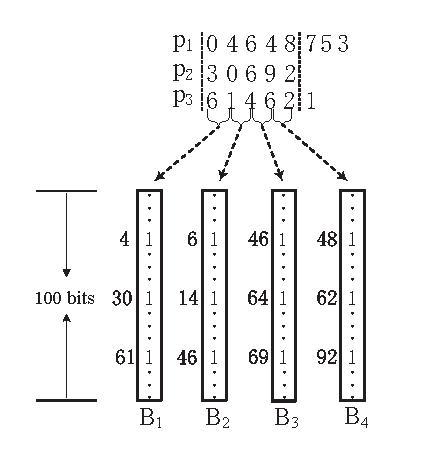
\includegraphics[height=2in, width=2in]{./eps/filter}
  \caption{为3个数字模式串所构造的过滤模块}
  \label{fig:filter}
\end{figure}

图 \ref{fig:filter} 给出了过滤模块的一个例子, 假设字符集为
$\Sigma = \{0, 1, 2, \dots, 9\}$, 且模式集为 $P = \{p_1,\; p_2,\;
p_3\}$, 其中 $p_1 = 04648753$, $p_2 = 30692$, $p_3 = 614621$. 很明显,
$lsp = |p_2|= 5$. 假设 $k = 2$, $N = 100$, 且哈希函数是恒同映射. 对于这
样的情况, 过滤模块将包含 $lsp - k + 1 = 4$ 个查询位图, 即 $B_1$,
$B_2$, $B_3$, $B_4$, 且其中有 $B_1[i] = 1$ 当且仅当 $i$ = 4, 30, or
61; $B_2[i] = 1$ 当且仅当 $i$ = 6, 14, or 46; $B_3[i] = 1$ 当且仅
当 $i$ = 46, 64, or 69; 以及 $B_4[i] = 1$ 当且仅当 $i$ = 48, 62, or
92.

一旦查询位图构造完成, 便可以用来过滤文本串中的位置. 在过滤操作中,一个长
为 $lsp$ 的滑动窗口 $W$ 被用来在文本串 $T$ 中选取子串. 最初,
$W$ 与 $T$ 的最左端对齐, 所以 $W$ 包含的 $T$ 的子串为 $T[1,lsp]$. 一般
地, 假设 $W$ 移动到 $T$ 的第 $i$ 个位置, 且 $W$ 中包含的子串
为 $T[i,lsp]$. 接着 $T[i,lsp]$ 末尾长为 $k$ 的字符块, 即 $T[i+lsp-k,
k]$ 被用作输入来查询所有的位图. 令单个比特位 $qb_j$ 为 $B_j$ 的输
出 ($1 \leq j \leq lsp - k + 1$), 且 $qb_j=1$ 当且仅
当 $B_j[hash(T[i+lsp-k,k])] = 1$. 令结果位图
$QB = qb_1qb_2 \dots qb_{lsp-k+1}$ 表示当前的查询结果, 用主位图
$MB = mb_1mb_2 \dots mb_{lsp-k+1}$ 来累加以前的查询结果, 并作为过滤模块
当前的状态向量. 最初, 主位图 $MB$ 的所有位都被设置为 1. 在得到一个查询
结果 $QB$ 之后, 主位图将被更新为 $MB = MB \; \& \; QB$, 其中 \& 是''按
位与''操作. 对于更新后的 $MB$, 如果 $mb_{lsp-k+1} = 1$, 则位置 $i$ 是一
个潜在匹配点, 且将激活核实模块. 否则, 滑动窗口 $W$ 将前进 $lsp-k+1$ 个
位置, 如果 $MB$ 所有的位都为 0; 或前进 $lsp-k+1-r$ 个位置, 若 $mb_r=1$
且 $mb_i=0$, $r < i \leq lsp-k$. 被滑动窗口 $W$ 跳过的位置都已经被过滤
掉.  如果 $W$ 将前进 $h$ 个位置, 则将 $MB$ 右移 $h$ 位且向左边空出来的
位补1. 值得注意的是, 在 \cite{Lee2013} 中作者已经证实, 过滤模块可以最大
化地利用以前的查询结果, 在滑动窗口每次前进的长度方面是最优的 (即可以过
滤掉尽可能多的位置).

\begin{figure}[htbp]
  \centering
  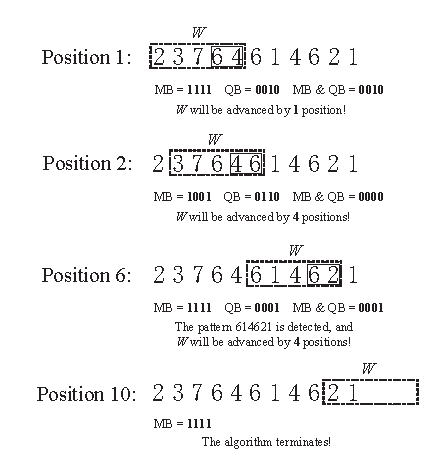
\includegraphics[height=2.5in, width=2.5in]{./eps/filter_match}
  \caption{使用过滤模块过滤文本中的非匹配位置.}
  \label{fig:f_match}
\end{figure}

举例说明, (见图 \ref{fig:f_match}), 考虑前面构造好的查询位图, 同时假
设 $T=23764614621$.  最初, 滑动窗口 $W$ 包含23764 且 $MB = 1111$.
23764末尾的长为2的字符块, 即64, 被用作第一次查询, 且查询结果
为 $QB=0010$. 由于 $MB\; \&\; QB = 0010$, $W$ 将前进一个位置 (即 $T$ 的
第一个位置已被过滤掉), 接着 $MB$ 会右移1位且左边补1, 变成 $1001$. 对于
第二个位置, $W$ 中所包含的子串为37646. 此时, 字符块46被用来查询位图, 查
询结果为 $QB=0110$. 由于 $MB\; \& \; QB=0000$, $W$ 将向前移动4个位置到
位置6 (第 $2 \sim 5$ 位被过滤掉了), 且 $MB$ 将被更新为1111. 对于位置6,
$W$ 包含61462, 字符块62将被用来进行查询得到 $QB = 0001$. 由于 $MB\; \&
\; QB = 0001$, 位置6是一个潜在匹配位置, 此时将激活核实模块. 经过核实,
模式串 $p_3=614621$ 出现于位置6. 接着, $W$ 向后移动4位到达位
置10. 然而, 由于此时 $W$ 中剩余子串的长度小于 $lsp$, 这意味着不可能再有
任何模式串出现, 因此, 整个算法结束.

\section{核实模块}
\label{sec:verification}

核实模块是整个匹配引擎的核心, 其决定了引擎性能的下界 (即最差性能). 核实
模块基于一种被称为自适应匹配树(AMT)的新型数据结构, 它是经典trie树结构的
一种改进. 类似于trie树, 但是以一种更加高效灵活的方式, AMT能够进行快速的
成员查询, 以此来决定给定字符串是否存在于模式集中. 接下来将介绍AMT的构建
方式, 和进一步的优化技术.

\subsection{构建AMT}
\label{subsec:amt}

AMT基于模式集构建, 总体来说, 构建过程包含以下5个主要步骤:

\begin{enumerate}
\item 创建后缀集 $SF$ 并将模式集中的所有模式串放入 $SF$. 每个模式串都视
  为它自身的一个后缀.
\item 计算 $SF$ 中最短后缀的长度, 用 $lss$表示. 对于 $SF$ 中的每一个后
  缀, 去掉其长为 $lss$ 的前缀, 所有被移除的前缀构成前缀
  集 $PF$. 对 $PF$ 进行去重, 同时计算 $|PF|$, 即不同前缀的数
  量, 用 $ndp$ 表示.
\item 产生一个树节点 $node$ 来保存 $PF$ 中的所有前缀. $node$ 本质上是一
  个索引结构, 以其所保存的前缀作为键. 节点 $node$ 的内部结构, 会根据上
  一步中计算出的 $ndp$ 和 $lss$ 进行自适应选择. 有多种结构可供选择.
\item 将 $SF$ 中具有相同(但已被移除的)前缀的后缀聚集起来, 形成子后缀
  集. 将每个子后缀集与其在 $node$ 中对应的前缀关联起来.
\item 对于上一步产生的每个子后缀集, 从步骤2开始, 重复执行同样的过程.直
  到不再产生新的子后缀集.
\end{enumerate}

\begin{figure}[htbp]
  \centering
  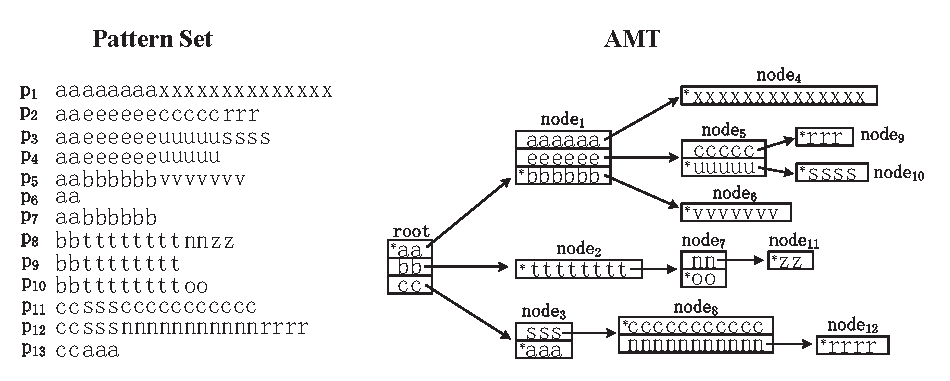
\includegraphics[width=\textwidth]{./eps/AMT}
  \caption{从模式集构造AMT. AMT中的每个箭头代表一个指向孩子节点的指针.}
  \label{fig:AMT}
\end{figure}

作为一个例子, 图 \ref{fig:AMT} 显示了从模式集
$P = \{p_1,\, p_2,\, \dots,\, p_{13}\}$ 构造AMT的过程。 注意, 由于每个
模式串都是自身的一个后缀, 模式集 $P$ 也可以被看作一个后缀集 $SF$. 首先,由
于 $p_6$ 是 $P$ 中最短的模式串(后缀), 所以 $lss = |p_6| = 2$. 接着,
移除掉每个模式串(后缀)长为2的前缀, 所有被移除掉的前缀构成了前缀集:
$PF = \{p_1^{+2} = aa,\; p_2^{+2} = aa,\; \dots,\; p_{13}^{+2} =
cc\}$.  在对 $PF$ 去重之后, 只剩下3个不同的前缀: $PF = \{aa,\, bb,\,
cc\}$, 同时有 $ndp = |PF| = 3$.

然后,产生AMT的第一个节点即根节点, 来存储 $PF$ 中的前缀。 每个前缀都作
为根节点中的一个键,并且具有一个指向其未来的孩子节点的指针(初始化为
空)。 正如稍后即将看到的, 根节点的结构将会根据两个参数:
$lss=2$ 和 $ndp=3$ 进行自适应选择。

在产生根节点之后, $P$ 中剩余的后缀将会根据其被去掉的(长为2的)前缀分成若
干组: 具有相同(被移除)前缀的那些后缀将分为一组,形成一个子后缀集。 同时,
使用二元组 (\emph{node.key,\; sub-suffix-set}) 来记录后缀与其被移除前缀
之前的联系: \emph{sub-suffix-set} 中的每个后缀都被移除掉了相同的前
缀 \emph{key}, \emph{key} 是新产生节点 \emph{node} 中的一个键. 使用这种
表示法, 在对 $P$ 中剩余的后缀分组之后, 会产生3个二元组:
$tp_1 = (root.aa,\; SF_1=\{p_1^{-2},\, p_2^{-2},\, p_3^{-2},\,
p_4^{-2},\, p_5^{-2},\, p_7^{-2}\})$,\,
$tp_2 = (root.bb,\; SF_2=\{p_8^{-2},\, p_9^{-2},\,
p_{10}^{-2}\})$ 和
$tp_3 = (root.cc,\; SF_3=\{p_{11}^{-2},\, p_{12}^{-2},\,
p_{13}^{-2}\})$. 即 $P$ 被分成了3个子模式集: $SF_1$, $SF_2$, $SF_3$, 分
别对应于根节点中的一个前缀 (这意味着根节点会有3个孩子节点). 注意, 最短
的后缀(模式串) $p_6$ 在子模式集中已经消失了, 因为在移除 $p_6$ 长为2的前
缀之后, $p_6$ 将不包含任何字符(即空串)。

同样的过程将会在3个新产生的子后缀集上重复. 作为进一步的例子, $tp_1$ 中
的 $SF_1$ 将会被处理. 首先, 由于 $lss = |p_7^{-2}| = 6$, $SF_1$ 中每个
后缀长为6的前缀将会被移除,并形成前缀集:
$PF_1 = \{(p_1^{-2})^{+6},\, (p_2^{-2})^{+6},\, (p_3^{-2})^{+6},\,
(p_4^{-2})^{+6},\, (p_5^{-2})^{+6},\, (p_7^{-2})^{+6}\}$. 在对 $PF_1$
去重之后, 仅剩余3个不同的前缀: $PF_1 = \{a^6,\, e^6,\, b^6\}$ (用符
号 $c^n$ 来表示由相同字符 $c$ 组成的长为 $n$ 的字符串).  然后,基
于 $PF_1$ 自适应地产生一个新的树节点 $node_1$ 来存储 $PF_1$ 中的前
缀。 根据 $tp_1$ 的第一个分量 (即 $root.aa$), $node_1$ 将会通过孩子指针
与根节点中的前缀 $aa$ 相关联, 使其成为根节点的第一个孩子节点. 再一次,
$SF_1$ 中的后缀将会根据它们被移除的长为6的前缀被分组,这会产生6个二元组:
$tp_4 = (node_1.a^6,\; SF_4=\{p_1^{-8}\})$,
$tp_5 = (node_1.e^6,\; SF_5=\{p_2^{-8},\, p_3^{-8},\,
p_4^{-8}\})$ 和 $tp_6 = (node_1.b^6,\; SF_6=\{p_5^{-8}\})$.

注意, 为了标记模式的终止, 一旦一个模式的最后一部分被移除并存储于某个树
节点中,相应节点中的该部分将会由星号标记. 这样, 任一从根节点到标记有星
号的节点的路径都代表了一个完整的模式串. 可以看到, 模式集中的所有模式串
都隐式地存储于 AMT中,并可由以上所提到的路径进行重建。

在构建AMT的过程中, 我们将使用广度优先策略来处理每个子后缀集并产生相应的
节点 (这意味着下一个待处理的子后缀集是 $SF_2$ 而非 $SF_4$). 为了记录子
后缀集处理的先后顺序, 将使用一个''先进先出''队列来保存产生的子后缀集所
对应的二元组. 位于队列首的二元组包含了下一个将要处理的子后缀集, 新生成
的子后缀集所对应的二元组将会依次插入到队列尾. 在本例中, 根节点最先被生
成, 接着 $tp_1$, $tp_2$ 和 $tp_3$ 将被依次插入队列. 然后 $tp_1$ 所包含
的 $SF_1$ 将被处理, 同时新产生的元组 $tp_4$, $tp_5$ 和 $tp_6$ 将被依次
插入到队列尾. 接下来, $SF_2$, $SF_3$, $SF_4$, $SF_5$, $SF_6$, $\dots$
将被依次处理. 一旦队列为空, AMT将构建完成. 值得指出的是, 同样可以使用深
度优先策略来逐分支的构造AMT, 但无论使用哪种策略, 最终构造出的AMT都是相
同的.


\begin{algorithm}
  \caption{构造AMT}\scriptsize
  \label{alg:amt}
  \begin{algorithmic}[1]
    \REQUIRE 模式集 $P$
    \ENSURE  相应的 AMT
    \STATE
    \STATE $Q \leftarrow$ 产生空队列
    \STATE $push\_queue((NULL,\,P),\; Q)$
    \STATE
    \WHILE{$Q \neq \emptyset$}
    \STATE $(parent\_node.key,\; SF) \leftarrow pop\_queue(Q)$
    \STATE $lss \leftarrow$ $SF$ 中最短后缀的长度
    \FOR{每一个 $suf \in SF$}
    \IF{$|suf|=lss$}
    \STATE 将 $suf^{+lss}$ 标记为模式终止处
    \ENDIF
    \STATE   从 $suf$ 移除 $suf^{+lss}$, 同时将 $suf^{+lss}$ 插入 $PF$
    \ENDFOR
    \STATE 对 $PF$ 去重, 令 $ndp \leftarrow |PF|$
    \STATE 根据 $lss$ 和 $ndp$, 自适应地产生新节点
    $new\_node$ 来存储 $PF$ 中的前缀
    \IF{$(parent\_node.key = NULL)$}
    \STATE $root \leftarrow new\_node$
    \ELSE
    \STATE 通过孩子指针将 $new\_node$
    与 $parent\_node.key$ 相关联
    \ENDIF
    \STATE $TP \leftarrow \{(new\_node.pf,\, SSF) \mid SSF \subseteq SF\; and
    \ \forall \ p,\,q \in SSF: p,\,q$ 具有相同的长为 $lss$ 的前缀
    $pf$ 被移除\}\
    \FOR{每一个 $tp \in TP$}
    \STATE $push\_queue(Q,\,tp)$
    \ENDFOR
    \ENDWHILE
    \STATE
    \RETURN $root$.
  \end{algorithmic}
\end{algorithm}

从模式集构造AMT的框架在算法 \ref{alg:amt} 中显示. 首先, 产生一个空队
列 $Q$ 来保存二元组 (第2行). 接着元组 $(NULL, P)$ 被函数 $push\_queue$
插入到 $Q$ 中(第3行), 其中 $push\_queue$ 总是将元素插入到队列
尾. 由于 $P$ 是初始模式集, 此时还没有任何前缀被移除, 所以上述元组的第一
个分量为空($NULL$). 这样, 根节点的产生过程就可以和其它节点一起被合并到
接下来的 \textbf{while} 循环中.

若 $Q$ 非空, 第5行到第25行的 \textbf{while} 循环将基于 $Q$ 的第一个元组
来产生节点. 位于 $Q$ 首的元组将由 $pop\_queue(Q)$ 函数取出(第6行): 将要
被处理的后缀集由 $SF$ 表示, $SF$ 在其父节点中所对应的前缀
由 $parent\_node.key$ 表示. 接着 $lss$ 和 $SF$ 将被计
算(第7行). 在第8到13行的内层 \textbf{for} 循环中, $SF$ 中每一个后缀的长
为 $lss$ 的前缀将被移除, 被移除的前缀构成前缀集 $PF$. 如果一个前缀是某
个模式串的最后一部分, 该前缀将被标记为模式终止. 然后会对 $PF$ 进行去
重 (第14行), 紧接着, 自适应地产生一个新的树节点来保存 $PF$ 中的前
缀 (第15行). 第16行中的 \textbf{if} 语句将判断新产生的节点是否是根节点:如
前所述, 若当前二元组的第一个分量为 $NULL$, 则新产生的节点为根节
点; 否则, 新节点将会与其父节点中的对应前缀相关联. 接下来(第21行), $SF$
中剩余的后缀将会根据其被移除的前缀进行分组, 每一组将与其对应前缀构成一
个二元组. 最后, 新产生的二元组将会依次插入到 $Q$ 的末尾. 一旦 $Q$ 没有
待处理二元组, 整个AMT将构建完成, 其根节点将被返回.

\subsection{核实}
\label{subsec:matching}

正如在过滤模块中所提到的, 一旦文本串中的潜在匹配位置被检测出, 核实模块
将会核实该位置是否有模式串出现. 具体地, 对一个潜在匹配位置 $i$, 核实模
块会将起始于 $i$ 的子串与AMT中(从根节点开始)的对应节点进行比对. 如果子
串成功匹配到某个标记为模式终止的节点, 那么可以断定存在模式串出现于位
置 $i$. 然而, 如果出现了匹配失败或匹配过程超出了AMT的叶节点, 匹配引擎将
会立刻前进到下一个位置 $i+1$, 同时再次激活过滤模块.

核实过程的伪代码, 在算法 \ref{alg:matching} 中描述. 假设 $i$ 是由过滤模
块检测出的文本串中的一个潜在匹配位置. 变量 $m\_len$ 是文本串中与AMT中节
点(中所包含的键)成功匹配的子串的总长度. 变量 $node$ 标识当前AMT中的正在
匹配的节点. 另外, 由于一个节点所包含的键(即前缀)具有相同的长
度, 符号 $key\_len(node)$ 用来表示节点 $node$ 中键的长度.

\begin{algorithm}
  \caption{核实过程}\scriptsize
  \label{alg:matching}
  \begin{algorithmic}[1]
    \REQUIRE ~~\\
    文本 $T$ 中的一个潜在匹配位置 $i$ \\
    基于模式集 $P$ 所构造的 AMT\\
    \ENSURE ~~\\
    起始于位置 $i$ 的所有模式串(如果存在)
    \STATE
    \STATE $m\_len \leftarrow 0$
    \STATE $node \leftarrow $ AMT的根节点
    \STATE
    \WHILE{$node \neq NULL$ and $\exists key \in node: key =
      T[i+m\_len, \, key\_len(node)]$}
    \STATE $m\_len \leftarrow m\_len + key\_len(node)$
    \IF{$key$ 被标记为模式终止}
    \STATE 输出: 模式串 $T[i,\,m\_len]$ 出现于位置 $i$
    \ENDIF
    \STATE $node \leftarrow$  $node$ 对应于 $node.key$ 的孩子节点
    \ENDWHILE
  \end{algorithmic}
\end{algorithm}

对于潜在匹配位置 $i$, 第5到11行的 \textbf{while} 循环将核实是否存在出现
于位置 $i$ 的模式串. 核实过程起始于AMT的根节点: 如果子文本
串 $T[i+m\_len, \, key\_len(node)]$ 匹配了当前节点 $node$ 中的某个
键 $key$, 成功匹配子串的总长度 $m\_len$ 将会增加 $key$ 的长度. 与此同
时, 如果 $key$ 也被标记为模式终止, 核实模块则会声称找到一个出现于 $i$
的模式串, 即 $T[i,\,m\_len]$. 接着, 核实过程将会转移到 $node.key$ 所对
应的孩子节点. 一旦出现了失配或当前节点超出了AMT的叶节点 (即 $node =
NULL$), 核实过程将终止, 匹配引擎会前进到下一个位置 $i+1$.

注意, 由于AMT中的节点有各自不同的内部结构, 在某个节点中搜索目标字符串
时, 必须使用对应于该节点类型的搜索函数.

\begin{figure}[htbp]
  \centering
  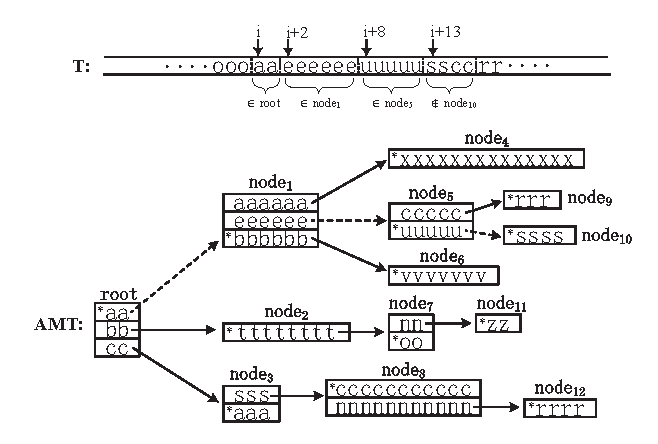
\includegraphics[width=0.75\textwidth]{./eps/match}
  \caption{对文本串中潜在匹配位置 $i$ 的核实过程.}
  \label{fig:matching}
\end{figure}

接下来, 将给出一个实例来说明如何使用 \ref{subsec:amt} 节所构造的AMT,对
文本串 $T$ 中的潜在匹配位置 $i$ 进行核实. 核实过程起始于AMT的根节点:根
据 $key\_len(root)=2$, 将起始于位置 $i$ 的同样长度的文本子
串, 即 $T[i,\,2]=aa$, 与根节点中的键进行匹配. 由于 $aa \in
root$ 且 $aa$ 被标记为模式终止. 所以模式串 $T[i,\,2]=aa$
(即 $P$ 中的 $p_6$) 出现于位置 $i$. 接着, 核实过程将转移到 $root.aa$ 所
对应的孩子节点.

对于节点 $node_1$, 由于 $key\_len(node_1)=6$, 同样长度的子
串 $T[i+2,\,6]=e^6$ (跟随在 $T[i,\,2]$ 之后) 将会与 $node_1$ 中的键进行
匹配. 由于 $e^6 \in node_1$, 且并非模式串结尾, 核实过程将转移
到 $node_1.e^6$ 所对应的孩子节点 $node_5$ 上。

在节点 $node_5$ 上, 由于接下来的子文本串 $T[i+8,\,5]=u^5 \in
node_5$ 且 $u^5$ 被标记为模式终止, 另一个模式串 $T[i,\,13]=a^2e^6u^5$
(即 $P$ 中的 $p_4$) 被发现于 $i$. 然后,核实过程将转移到 $node_5.u^5$
所应的孩子节点 $node_{10}$ 中。

在 $node_{10}$ 上, 由于 $T[i+13,\,4]=sscc \notin node_{10}$, 对位
置 $i$ 的核实过程将终止。 接下来, 匹配引擎将转移到下一个位置 $i+1$, 同
时激活过滤模块。

从以上过程可以看到, 对潜在匹配位置的核实过程对应于AMT中的一条“核实路
径”, 其中的节点都参与过与文本串的比较。 本例中, 位置 $i$ 所对应的核实
路径为:
$root \rightarrow node_1 \rightarrow node_5 \rightarrow node_{10}$, 由
图 \ref{fig:matching} 中的虚线箭头表示.


\subsection{自适应地产生树节点}
\label{subsec:nodes}

如 \ref{subsec:amt} 节所说的, AMT中的每个节点都有其特定的索引结构用来保
存前缀集中的前缀. 索引结构的类型将根据前缀集的特性自适应地进行选择. 由
于前缀集中的所有前缀(键)都具有相同的长度, 前缀集的特性主要可以由两个参
数进行刻画,即前缀集所包含前缀(键)的长度和数量. 这两个参数分别
由 \ref{subsec:amt} 节中的 $lss$ 和 $ndp$ 来表示.

有三种不同的结构, 即字符映射表, 字符串数组及哈希表可以用来作为树节点来
存储具有不同 $lss$ 和 $ndp$ 的前缀集. 接下来,将详细讨论这几种节点结构.

\subsubsection{字符映射表}

给定前缀集, 如果其前缀长度都为1 ($lss=1$), 即每一个前缀都是单个字符, 则
选用空间高效的字符映射表(由 Leis \cite{Leis2013} 提出)作为树节点. 对于
不同的前缀数 (即 $ndp$, $1 \leq ndp \leq 256$),有四种不同容量的字符映
射表可供选择。

\begin{figure}[hp]
  \centering
  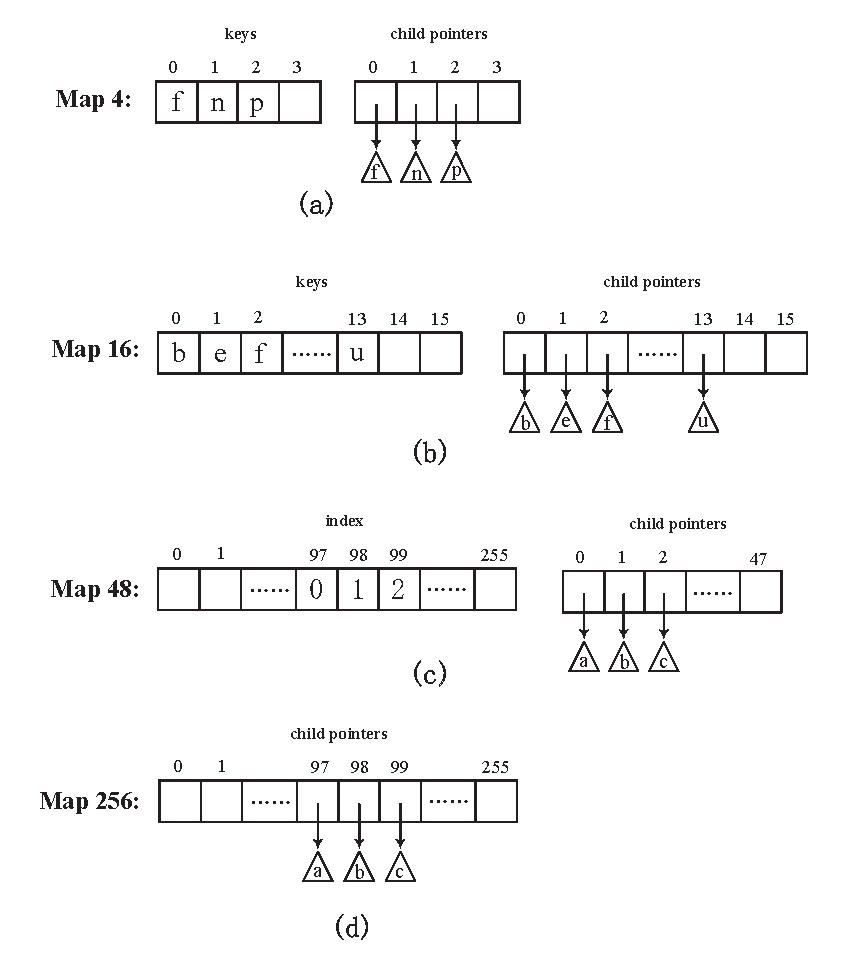
\includegraphics[height=3.5in, width=3.5in]{./eps/Maps}
  \caption{四种不同容量的字符映射表. 三角形代表相应键的子节点.}
  \label{fig:character map}
\end{figure}

图 \ref{fig:character map} 显示了由其最大容量所命名的四种字符映射表. 字
符映射表的键和其所对应的孩子指针,分别存放于两个不同的数组中,而非使用
二元组 (\emph{键, 孩子指针}) 数组, 这样能在保证高效匹配的同时保持节点的
紧凑。

\begin{itemize}
\item \textbf{Map 4} (当 $1 \leq ndp \leq 4$ 时采用): 这种最小的字符映
  射表最多能存储4个键。 它使用4个元素的数组来存储键,用另一个同样长度的
  数组来存储孩子指针。 键及其所对应的孩子指针存储在各自数组的相同位置,
  键按照其ASCII码值顺序存储. 一旦目标字符在键数组中被找到, 其所对于的孩
  子指针可在另一个数组的同样位置找到.  图 \ref{fig:character map} (a)
  显示了包含了3键:$f$, $n$ 和 $p$ 的 Map 4 结构,其中包含了键的三角形
  表示对应的孩子节点。

\item \textbf{Map 16} (当 $5 \leq ndp \leq 16$ 时采用): 这种字符映射表
  可以存储5到16个键. 它与Map 4映射表有类似的结构, 但两个数组都扩大到
  了16个元素. 目标字符可由键数组上的二分查找进行快速检
  索。 图 \ref{fig:character map} (b) 显示了具有14个键的 Map 16 映射
  表。


\item \textbf{Map 48} (当 $17 \leq ndp \leq 48$ 时采用): 随着键数量的增
  加, 在键数组中查找目标字符将变得越来越耗时。 因此, 当键的数量超过16个
  (但小于49个)时,将不再显示地存储键, 而是使用一个具有256个元素的索引
  数组,该数组可由目标字符的ASCII码值作为下标直接访问其元素。 索引数组
  存储的是另外一个具有48个元素的孩子指针数组的索引(下标)(在$[0,47]$范
  围内的整数)。 相比直接存储孩子指针,这种方式更加节省空间, 因为每个数
  组下标只占用一个字节的空间。 图 \ref{fig:character map} (c) 显示了一
  个Map 48映射表, 其中字符 $a$, $b$, $c$ 的ASCII码值分别为 97, 98, 99.

\item \textbf{Map 256} (当 $49 \leq ndp \leq 256$ 时采用): 最大的字符映
  射表只包含一个具有256个元素的数组来直接存储孩子指针,其中每个元素被初
  始化为 $NULL$. 当键的数量在49到256之间时,采用该类型的映射表作为树节
  点. 对于Map 256映射表, 相应的孩子节点可直接通过目标字符的ASCII码值找
  到. 与其他类型的映射表不同, Map 256只包含一个数组, 因此无需进行数组
  的二次访问, 而且,如果所包含数组大部分元素非空, 该结构同样非常紧
  凑. 图 \ref{fig:character map} (d) 显示了一个Map 256映射表, 其中只有
  一个指针数组。
\end{itemize}

在类型为字符映射表的节点中搜索目标字符的具体操作由算
法 \ref{alg:character map} 给出.

\begin{algorithm}
  \caption{在类型为字符映射表的节点中进行搜索}\scriptsize
  \label{alg:character map}
  \begin{algorithmic}[1]
    \REQUIRE ~~\\
    类型为字符映射表的节点 $node$\\
    目标字符 $t\_ch$.
    \ENSURE ~~\\
     $node.t\_ch$ 所对应的孩子节点 (可能为 $NULL$).
    \STATE
    \STATE $count \leftarrow$ 字符映射表中的键的个数
    \STATE
    \SWITCH{字符映射表的类型}
    \CASE{\textsf{Map 4}}
    \FOR{$i \leftarrow 0$ to $count-1$}
    \IF{$keys[i]=t\_ch$}
    \RETURN $child\_pointers[i]$
    \ENDIF
    \ENDFOR
    \STATE 出现失配,返回 $NULL$.
    \ENDCASE
    \STATE
    \CASE{\textsf{Map 16}}
    \STATE $low \leftarrow 0, high \leftarrow count-1$
    \WHILE{$low \le high$}
    \STATE $mid \leftarrow \lfloor (low+high)/2 \rfloor$
    \IF{$t\_ch=keys[mid]$}
    \RETURN $child\_pointers[mid]$
    \ELSIF{$t\_ch<keys[mid]$}
    \STATE $high \leftarrow mid-1$
    \ELSE
    \STATE $low \leftarrow mid+1$
    \ENDIF
    \ENDWHILE
    \STATE 出现失配,返回 $NULL$.
    \ENDCASE
    \STATE
    \CASE{\textsf{Map 48}}
    \IF{$index[t\_ch] \neq NULL$}
    \RETURN $child\_pointers[index[t\_ch]]$
    \ELSE
    \STATE 出现失配,返回 $NULL$.
    \ENDIF
    \ENDCASE
    \STATE
    \CASE{\textsf{Map 256}}
    \RETURN $child\_pointers[t\_ch]$
    \ENDCASE
    \ENDPWITCH
  \end{algorithmic}
\end{algorithm}

\subsubsection{字符串数组}
\label{sec:string array}

对于键长大于1 (即 $lss > 1$) 且键数不超过100 (即 $ndp \leq 100$)的前缀
集, 将选用字符串数组作为树节点来存储其中的键. 类似于 Map 4 和 Map 16 结
构, 键按照字典序存储在一个大小为 $ndp \times lss$ 字节的数组中, 每个键
占用 $lss$ 字节. 孩子指针存储在另一个数组的对应位置
上. 图 \ref{fig:string array} 显示了包含了3个键: $aaa$, $bbb$ 和 $ccc$
的字符串数组结构。

\begin{figure}[htbp]
  \centering
  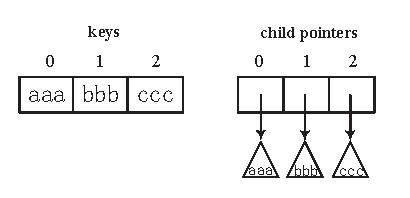
\includegraphics[width=0.45\textwidth]{./eps/string_array}
  \caption{包含3个键 $aaa,\, bbb,\, ccc$ 的字符串数组结构.}
  \label{fig:string array}
\end{figure}

为了高效起见, 如果键的数量小于5个, 则在键数组上使用简单的线性查找算法来
搜索目标字符串; 否则, 将采用更高效的 (也更为复杂的) 二分查找算
法. 算法 \ref{alg:string array} 显示了在类型为字符串数组的节点中搜索目
标字符串的过程,其中 $A \prec B$ 表示字符串 $A$ 以字典序小于字符
串 $B$. 对于包含小于5个键的字符串数组, 目标字符串将按顺序与键数组中的元
素依次比较. 如果目标字符串匹配了某个键, 返回指针数组中对应位置所包含的
孩子节点指针; 否则, 将出现失配. 另一方面, 如果键的数量大于4, 将使用二分
查找算法从键数组的中间元素开始, 搜索目标字符串。

\begin{algorithm}
  \caption{在类型为字符串数组的节点中搜索}\scriptsize
  \label{alg:string array}
  \begin{algorithmic}[1]
    \REQUIRE ~~\\
    类型为字符串数组的节点 $node$; \\
    目标字符串 $t\_str$.\\
    \ENSURE ~~\\
     $node.t\_ch$ 所对应的孩子节点 (可能为 $NULL$).\\
    \STATE
    \STATE $count \leftarrow$ 节点 $node$  所包含的键数
    \STATE
    \IF{$count < 5$}
    \STATE $i \leftarrow 0$
    \WHILE{$i < count$ 且 $keys[i] \prec t\_str$}
    \STATE $i \leftarrow i+1$
    \ENDWHILE
    \IF{$i < count$ 且 $keys[i]=t\_str$}
    \RETURN $child\_pointers[i]$
    \ELSE
    \STATE 出现失配,返回 $NULL$.
    \ENDIF
    \ELSE
    \STATE $low \leftarrow 0$, $high \leftarrow count-1$
    \WHILE{$low \leq high$}
    \STATE $mid \leftarrow \lfloor (low+high)/2 \rfloor$
    \IF{$t\_str = keys[mid]$}
    \RETURN $child\_pointers[mid]$
    \ELSIF{$t\_str < keys[mid]$}
    \STATE $high \leftarrow mid - 1$
    \ELSE
    \STATE $low \leftarrow mid + 1$
    \ENDIF
    \ENDWHILE
    \STATE 出现失配,返回 $NULL$.
    \ENDIF
  \end{algorithmic}
\end{algorithm}

\subsubsection{哈希表}
\label{sec:hash table}

对于键数大于100的前缀集 (即 $lss > 1$ 且 $ndp > 100$), 即使在字符串数组
上使用二分查找算法也不够高效。 此时, 将采用一种更快 (也更大)的数据结
构 --- 哈希表, 来处理包含大量键的情况. 值得注意的是, 哈希表是直接基于后
缀集构建的, 而不是像其他节点结构那样基于(从后缀集中生成的)的前缀集. 在
我们的实现中, 哈希表是一个孩子指针数组, 其中所有元素初始化为 $NULL$, 同
时, 配合使用一个字符串哈希函数, 该函数能将字符串转化为正整数.

具体地说, 给定后缀集 $SF$, 哈希表的长度(即元素个数, 由 $table\_size$ 表
示) 由 $ndp$ 和一个给定的负载因子 $lf$
(即 $ndp$ 与 $table\_size$ 比值) 决定, 即.
$table\_size = \lceil ndp\,/\,lf \rceil$. 例如, 给定 $ndp =
1000$ 及 $lf = 70\%$, 则哈希表的长度为
$table\_size = \lceil 1000/0.7 \rceil = 1429$. 注意, 这里的 $ndp$ 被定
义为后缀集 $SF$ 中, 后缀所包含的长为 $lss$ 的不同前缀的数量, 这与去重后
的前缀集 $PF$ 所包含的前缀数相同.

算法 \ref{alg:hash} 显示了基于后缀集 $SF$ 构建哈希表的过程.  首先,
$SF$ 将会基于哈希值被分为若干个子后缀集: 对于每个后缀 $suf \in SF$, 它
的前缀 $suf^{+lss}$ 将通过哈希函数转化为一个 0 到 $table\_size-1$ 之间
的整数 $i$, 然后 $suf$ 将与哈希表第 $i$ 个元素相关联. 此后, 那些长
为 $lss$ 的前缀被哈希到同一个值的后缀将与哈希表的同一个元素相关联, 构成
一个子后缀集. 接着, 为了解决哈希冲突, 对于哈希表中每个非 $NULL$ 元素所
关联的子后缀集 $SSF$, 构造其相应的前缀集, 然后按照算
法 \ref{alg:amt} 中 \textbf{while} 循环所示, 构造相应的树节点. 新产生的
树节点将会取代子后缀集与相应的哈希表元素关联. 这样, 会有许多不同结构的
节点关联到同一个哈希表上.

% The suffixes whose length-$lss$ prefixes hashed to the same
% value $i$ are collected together associated with the $i$-th bucket and
% forms a small suffix set. (Note that, we do not remove the prefixes of
% the suffixes when partitioning $SF$.) Then, to address the collisions,
% for each non-$NULL$ bucket of the hash table, a tree node is built based
% on the small suffix set associated with that bucket as stated
% before. Hence, many tree nodes with various structures can be
% incorporated in one hash table.


\begin{algorithm}
  \caption{构建哈希表}\scriptsize
  \label{alg:hash}
  \begin{algorithmic}[1]
    \REQUIRE ~~\\
    后缀集 $SF$ 及负载因子 $lf$. \\
    \ENSURE ~~\\
    哈希表.\\
    \STATE
    \STATE $ndp \leftarrow$ $SF$ 中, 后缀所具有的长为 $lss$ 的不同前缀
    的数量.
    \STATE $table\_size \leftarrow \lceil ndp\,/\,lf \rceil$
    \STATE $hash\_table \leftarrow$ 产生一个具有
    $table\_size$ 个孩子指针的数组, 每个指针被初始化为 $NULL$.
    \STATE
    \FOR{每一个 $suf \in SF$}
    \STATE $i \leftarrow Hash(suf^{+lss})$
    \STATE 将 $suf$ 与 $hash\_table[i]$ 相关联
    \ENDFOR
    \STATE
    \FOR{$i \leftarrow 0$ to $table\_size - 1$}
    \IF{$hash\_table[i]\, \neq\, NULL$}
    \STATE $SSF \leftarrow \{suf\,|\,suf\in SF\; and\; Hash(suf^{+lss})=i\}$
    \STATE $new\_node \leftarrow$ 如算法 \ref{alg:amt} 中的
    \textbf{while} 循环所示, 基于 $SSF$ 自适应地产生一个树节点.
    \STATE 将 $new\_node$ 与 $hash\_table[i]$ 相关联.
    \ENDIF
    \ENDFOR
    \STATE
    \RETURN $hash\_table$
  \end{algorithmic}
\end{algorithm}

给定长为 $lss$ 目标字符串, 首先计算其哈希值并将哈希值用作哈希表的数组下
标. 如果哈希表对应元素为 $NULL$, 意味着出现失配, 将终止核实过程并转移到
文本的下一个位置; 否则, 核实过程将转移到与其关联的孩子节点中.

哈希表所采用的字符串哈希函数, 将会很大程度地影响匹配的效率. 在我们的实
现中, 对于每一次匹配任务, 将从一个哈希函数族 $H$ 中随机地选取一个哈希函
数. 所采用的哈希函数来自于 Ramakrishna \cite{Ramakrishna1997} 所提出
的 \emph{shift-add-xor} 哈希函数族, 该哈希函数族具有良好的均匀性和一致
性.

\subsection{进一步优化}
\label{sec:further improments}

以上介绍的核实模块已经相当高效, 但是仍然有一些技术可以进一步提升其时间
和空间效率。

\subsubsection{分解AMT}
\label{sec:divide amt}

以上介绍的核实模块基于由整个模式集所构建的AMT. 事实上, 可以将大的AMT分
解为多个小AMT, 同时让每一次核实操作只关联其中一个小AMT, 这样可以进一步
提高核实过程的效率. 分解过程基于以下思路。

如 \ref{sec:filter} 所述, 过滤过程基于滑动窗口所包含子串末尾的 $k$ 字符
块. 对于文本串 $T$ 的一个位置 $i$, 若某个模式串 $p_j$ 出现于 $i$, 则一
定有 $Hash[T[i+lss-k,k]] = Hash[p_j[lss-k+1,k]]$
($Hash[p_j[lss-k+1,k]]$ 被称为 $p_j$ 的标签值). 这意味着,可以根据标签
值将模式串进行分组:具有相同标签值的模式串被分成一组,构成一个子模式
集。 然后,为每一个子模式集构造一棵(小的)AMT。 另外, 还需构建一个索引表
使得相应的AMT可以由其对应的标签值在 $O(1)$ 时间内找到. 这样, 核实模块将
包含一个索引表和若干个(小的)AMT。

在过滤阶段, 一旦 $T$ 中的一个潜在匹配位置 $i$ 被找到, 将计算哈希
值 $Hash[T[i+lss-k,k]]$ 并将其用作索引表的索引来找到对应的AMT。 由于
该AMT的规模相比之前减小了,核实所用的时间也会相应地减少。

\subsubsection{节点合并}
\label{sec:node merge}

类似于Trie树结构中广泛使用的路径压缩技术,在AMT中的一条路径上,所有只包
含一个键的节点可以合并为一个节点。 该技术可以从时间和空间两方面提
高AMT的效率。 为了说明该技术的优势, 考虑模式集
$P=\{p_1=e^6u^5sscc,\; p_2=e^6u^5,\; p_3=e^6\}$ 和其所对应
的AMT。 如图 \ref{fig:merge} 所示, 所构建的AMT包含3个节点, 每个节点都只
有一个键. 在 x86\_64 体系结构中, 这种实现方法大致需要55字节的存储空间:
存储3个键需要15字节, 2个孩子指针需要16字节, 3个指向各自匹配函数的函数
指针需要24字节。 然而, 如果将3个键连接成1个字符串, 这3个节点便可合并
为1个, 这样不仅不再需要孩子指针,指向匹配函数的指针也从3个减少为1个。合
并后的节点构成一种新的节点结构,有别于 \ref{subsec:nodes} 节介绍的几种
节点类型.

\begin{figure}[htbp]
  \centering
  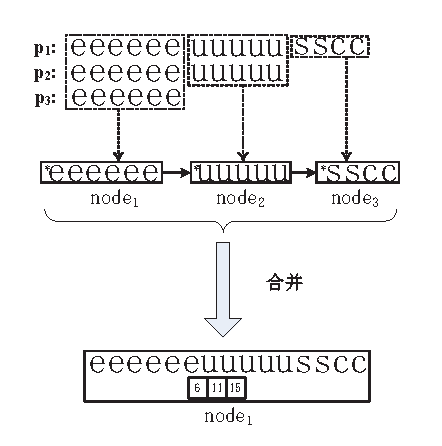
\includegraphics[height=2in, width=2in]{./eps/node_merge}
  \caption{节点合并.}
  \label{fig:merge}
\end{figure}

对于合并后的节点, 唯一的问题是如何区分被连接在一起的键。 为此, 需要使用
一个长度数组来记录每个键的长度,其中每个数组元素占用一个字
节 (使用 \emph{unsigned char} 类型). 通过每个键的长度,便可以识别出每个
键,这样,在合并后的节点中搜索目标字符串就变的很容易。

综上, 在节点合并之后, AMT只包含一个合并后的节点,且只占用26字节的存储空
间 (15个字节用来存储键, 3个字节用来存储长度数组, 8个字节用来存储指向匹
配函数的指针), 这样, 相比原先的AMT,合并节点后的AMT可以节省29个字节的存
储空间。 另外, 只需要一次随机访问内存便可以取出需要的节点, 相比原先需
要三次访问内存来取得需要的节点, 减少了内存访问量,提高了匹配速度。


\subsubsection{节点分割}
\label{sec:node split}

为了进一步提高节点的匹配效率, 一旦某个节点所包含的键具有公共前缀, 该前
缀便可以从节点中分离出来形成一个(包含单个键的)新节点。 (由于被分离出的
前缀是一个字符串或字符,新节点的结构只能是Map 4字符映射表或字符串数
组)。 在一个节点上搜索目标串时,节点分割技术可以大幅减少不必要的比较操
作。 例如, 如图 \ref{fig:split} 所示, 考虑在一个类型为字符串数组的节点
中搜索目标字符串 $a^5u$, 节点中的4个键具有公共前缀 $a^5$. 根据算
法 \ref{alg:string array}, 目标字符串需要与这4个键依次进行逐字符比较才
能确认其是否匹配某个键,这总共需要 $6 \times 4 = 24$ 次比较操作。 然而,如
果公共前缀 $a^5$ 被分离出来并形成一个新的节点,如图 \ref{fig:split} 所
示, 对于同样的目标字符串, 只需要9次字节比较操作便可以最终确
认 ($node_1$ 上需要5次比较, $node_2$ 上需要4次比较). 很明显, 通过对原
先的节点进行分割,减少了15次比较操作。

\begin{figure}[htbp]
  \centering
  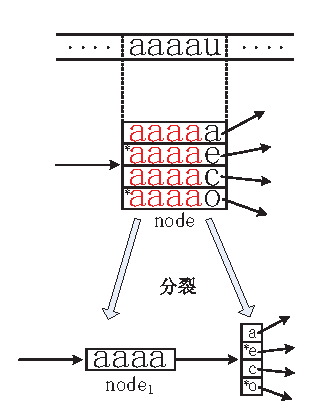
\includegraphics[height=2.5in, width=2in]{./eps/node_split}
  \caption{节点分割.}
  \label{fig:split}
\end{figure}



\section{实验结果}
\label{sec:experiments}

在本节中, 我们将所提出的匹配引擎(Fast Engine for MPM, 简称
为\textsf{FEMPM}) 与其他5个算法进行比较,来评估匹配引擎的性能。 参与比
较的算法包括: 2个经典的MPM基准算法 \textsf{AC} 和 \textsf{WM} ; 3个近
期提出的高效算法 \textsf{Split},
\textsf{MASM} 及 \textsf{Pre-filter+AC}. 所有算法都从两个方面对其性能进
行评估: 通过具有不同 $lsp$ 的模式集,来测试算法的鲁棒性;通过包含不同数
量模式的模式集来测试算法的可伸缩性。

\subsection{实验设置}


实验在一台PC上进行,配置有 Intel core i7 2.93GHz CPU, 8GB 内存 和 1TB硬
盘, 操作系统为GNU/Linux. 所有算法以 C/C++ 实现, gcc编译(-O2)。 测试数
据为来自于 Pizza\;\&\;Chili 语料库 (http://pizzachil.dcc.uchile.cl) 的
真实英文文本. 模式串从文本串中随机抽取,构成模式集。

实验过程中, \textsf{FEMPM} 的参数设置如下: 对于字符串数组, 如果其包
含的键数大于4, 则在键数组上使用二分查找来搜索目标字符串; 否则, 将使用
简单的线性查找算法 (对于包含小于4个键的字符串数组,线性查找算法由于其简
单性,反而更加高效). 对于哈希表, 为了平衡时间效率和空间效率,负载因子被
设置为 {0.5}; 产生哈希函数的种子值在 1~50 间随机产生; 左移值 L 和右移
值 R 分别被设置为 \textbf{2} 和 \textbf{6} (有关哈希函数的参数都选
自 \cite{Ramakrishna1997}). 一旦 $ndp$ 大于 \textbf{100}, 将选用哈希表
来取代字符串数组作为节点结构. 所有这些选择的参数都在大量模式集上进行了
广泛的实验,在实际中被证实是高效的。

\subsection{鲁棒性评估}

正如前面提到过的, 许多MPM算法对于模式集的最短模式串长(即$lsp$)非常敏
感. 所以,有必要测试 \textsf{FEMPM} 引擎和其它算法在具有不同 $lsp$ 模式
集下的鲁棒性。 共有9个模式集参与测试,其 $lsp$从2递增到10,每个模式集都
包含$10^5$个模式串. 文本串的大小固定为 200 MB. 测试模式集的特征在
表 \ref{tab:lsps} 中列出, 包括: 最短模式串长 (LSP), 最长模式串
长 (LLP), 模式串的平均长度 (ALP), 模式串长的标准差 (SD), 模式串总
长 (TLP) 和模式串的数量 (Count).

\begin{figure}[htbp]
  \centering
  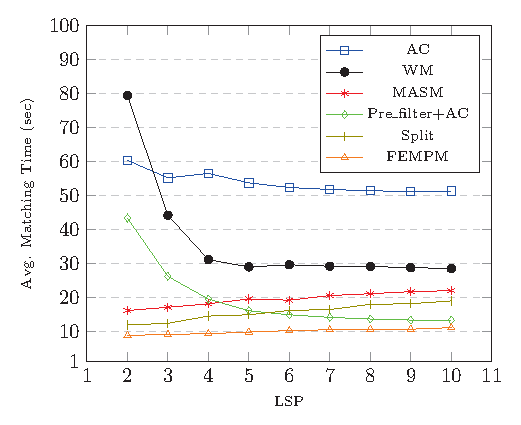
\includegraphics[height=2in, width=2.5in]{./eps/lsp}
  \caption{测试算法在具有不同lsp模式集下的匹配时间.}
  \label{fig:lsp}
\end{figure}


\begin{table}
  \centering
  \caption{测试模式集的特性.}
  \scriptsize
  \label{tab:lsps}
  \begin{tabular}{p{20pt}p{10pt}p{10pt}p{10pt}p{10pt}p{30pt}p{20pt}}
    \hline
    Pattern Set & LSP  & LLP  & ALP & SD & TLP & Count\\
    \hline
    $P_1$ & 2 & 50 & 25.9 & 14.1 & 2,599,020 & $10^5$\\
    $P_2$ & 3 & 50 & 26.5 & 13.9 & 2,646,762 & $10^5$\\
    $P_3$ & 4 & 50 & 27.0 & 13.6 & 2,704,091 & $10^5$\\
    $P_4$ & 5 & 50 & 27.6 & 13.2 & 2,745,545 & $10^5$\\
    $P_5$ & 6 & 50 & 27.9 & 13.0 & 2,793,178 & $10^5$\\
    $P_6$ & 7 & 50 & 28.4 & 12.7 & 2,843,580 & $10^5$\\
    $P_7$ & 8 & 50 & 29.0 & 12.4 & 2,903,343 & $10^5$\\
    $P_8$ & 9 & 50 & 29.5 & 12.1 & 2,948,372 & $10^5$\\
    $P_9$ &10 & 50 & 30.0 & 11.8 & 2,998,992 & $10^5$\\
    \hline
  \end{tabular}
\end{table}


图 \ref{fig:lsp} 给出了每个测试算法在独立运行5次后的平均运行时间(以秒位
单位). 总体来说, \textsf{AC} 算法受 $lsp$ 变化的影响不大。 但是, 其所构
建的DFA会消耗大量存储空间。 更糟糕的是, 算法在运行过程中会进行大量且不
可预测的状态转移,这会造成严重的cache miss,从而影响算法性能. 另一方
面, 同样基于DFA的 \textsf{Split} 算法, 对 $lsp$ 的变化也不敏感, 而且由
于它从模式集中抽取了一个子集来构造DFA,同时使用了位分割技术, 使其空间和
时间消耗都有大幅下降. 由图 \ref{fig:lsp} 可以看出,\textsf{WM} 算法的性
能受 $lsp$ 变化的影响很大: 对于 $lsp > 2$ 时,其性能优于AC, 但是对于包
含极短模式的模式集($lsp=2$),WM算法的性能将严重下降。 这是由于WM算法所
用的跳转策略并不适用于包含很短模式串的模式集,这意味着文本串中大部分位
置都无法被略过,而需要通过WM算法的哈希表进行二次检查,这将花费大量的时
间.  \textsf{Pre-filter+AC} 算法对于 $lsp > 5$ 的模式集的性能优于除
了 \textsf{FEMPM} 之外的其它算法。 该算法使用了类似的跳转策略: 一旦文本
串中的某个位置被Pre-filter过滤掉了, 其后最多有$lsp-1$个位置可以被跳
过. 因此, 对于 $lsp$ 较小的模式集, 文本中的大部分位置都无法被跳过, 这会
严重影响算法性能. 相比之下, \textsf{MASM} 算法对于较小 $lsp$ ($lsp
\leq 4$) 的模式集表现良好. 该算法首先通过前缀树结构对模式集进行压缩: 如
果模式串 $A$ 是另外一个模式串 $B$ 的前缀, $A$ 便可以合并到 $B$ 中. 然后,
算法将基于字典序为压缩后的模式集构造一棵二叉查找树。 相比长模式串, 短模
式串更有可能成为其它模式的前缀,因此, 更有可能被合并到其它串中. 因此,拥
有较小 $lsp$ 的模式集能被更好的压缩, 使得算法在匹配阶段的效率更高。

从图 \ref{fig:lsp} 可以看出, 我们所提出的 \textsf{FEMPM} 匹配引擎,对于
任何 $lsp$ 都拥有最佳的性能. 相比 \textsf{AC}, 对所有 $lsp$,匹配时间平
均减少了 $85\%$; 与更加高效的\textsf{Pre-filter+AC} 算法相比, 对于中等
长度的 $lsp$ ($lsp \geq 4$) 匹配时间减少了 $10\% \sim 20\%$, 对于较小
的 $lsp$ ($lsp < 4$), 匹配时间减少了 $70\%$. 尽管 \textsf{FEMPM} 的过滤
模块(和\textsf{Pre-filter+AC}类似), 同样不适用于较小的 $lsp$, 然而其核
实模块(即AMT), 相比 \textsf{Pre-filter+AC}的要更加高效. 这主要是由
于AMT节点的自适应性, 使得对于任何 $lsp$,所构造的AMT都能根据模式集的特
性自适应地调整到最优结构。得益于此, \textsf{FEMPM} 对于所有的测试模式集
都有最好的鲁棒性。 表 \ref{tab:node types} 中列出了不同模式集对应AMT中
节点类型的统计信息。 其中 Map 1 和 Single String Array 结构分别是 Map
4 和String Array结构只包含一个元素的特殊情形。 由此可以看出, 随着模式
集 $lsp$ 的变化, 对应AMT中的节点类型也会发生很大变化,这反映了AMT的自适
应性。

再者, \textsf{FEMPM} 的性能非常稳定可靠. 一旦文本的长度和模式串的数量确
定, 算法的运行时间对于不同 $lsp$ 的模式集,变化很
小. 如图 \ref{fig:lsp} 所示, 给定大小为200MB的文本和$10^5$个模式串,对
于不同的 $lsp$, \textsf{FEMPM} 的匹配时间大致都保持
在10s左右; 当 $lsp$从2递增到10时, 匹配时间的变化不超过2s. 事实
上, 随着$lsp$ 的增加, AMT中从根节点到叶节点路径的平均长度将会轻微地增
加. 相应地, 对于文本串中的某些位置,其对应的核实路径会增长,这会轻微地
影响算法的速度。

\begin{table}[!htp]
  \centering
  \caption{不同lsp模式集所对应AMT的节点类型统计}
  \scriptsize
  \label{tab:node types}
  \begin{tabular}{p{10pt}p{15pt}p{15pt}p{15pt}p{15pt}p{15pt}p{25pt}p{25pt}p{20pt}p{25pt}}
 \hline
 Lsp &
 Map 1 &
 Map 4 &
 Map 16 &
 Map 48 &
 Map 256 &
 Single String Array &
 String Array   &
 Hash Table &
 Total\\
 \hline
 2  & 2,464 & 2,096 & 663 & 133 & 0 & 63,274 &  21,627 & 10 & 90,267\\
 3  & 2,379 & 1,636 & 385 & 90  & 0 & 64,701 &  22,551 & 10 & 91,752\\
 4  & 2,273 & 1,329 & 201 & 57  & 0 & 66,162 &  22,736 &  1 & 92,759\\
 5  & 2,045 & 1,104 & 112 & 45  & 0 & 68,152 &  22,048 &  1 & 93,507\\
 6  & 1,758 &   899 &  52 & 34  & 0 & 70,179 &  20,818 &  1 & 93,741\\
 7  & 1,560 &   807 &  29 & 33  & 0 & 72,284 &  19,280 &  1 & 93,994\\
 8  & 1,515 &   803 &  20 & 31  & 0 & 73,447 &  18,274 &  1 & 94,091\\
 9  & 1,441 &   788 &  24 & 30  & 0 & 74,584 &  17,120 &  1 & 93,988\\
10  & 1,361 &   794 &  24 & 29  & 0 & 75,094 &  16,427 &  1 & 93,730\\
\hline
  \end{tabular}
\end{table}

\subsection{伸缩性评估}

本节将评估各种算法在不同容量模式集下的可伸缩性。 和前面一样, 文本串被固
定为200MB, 有两组模式集用于测试. 其中较小的一组包含9个模式集, 对应的模
式串数量由$1 \times 10^5$ 增加到 $9 \times 10^5$, 每次的增幅
为 $10^5$, 而较大的一组包含10个模式集, 对应模式串的数量由$10^6$ 增加
到 $10^7$,每次增加 $10^6$. 所有模式集的串长变化范围固定为 $5 \sim
50$.


\begin{figure}[htbp]
  \centering
  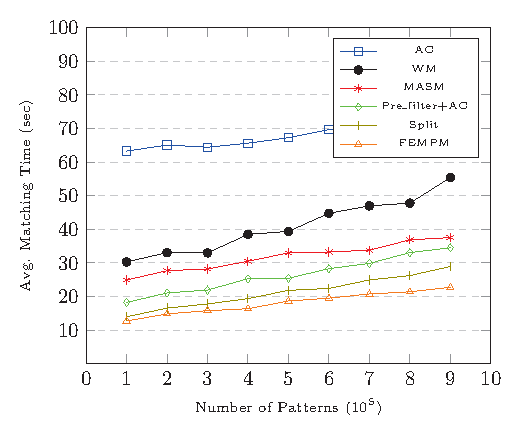
\includegraphics[height=2in, width=2.5in]{./eps/small_group}
  \caption{测试算法对于较小一组模式集的平均运行时间.}
  \label{fig:small_group}
\end{figure}

对于较小的一组模式集, 每个测试算法在每个模式集上独立运行5次,其平均运行
时间如图 \ref{fig:small_group} 所示. 实验结果表明, 随着模式串数量的增
加,AC算法的性能较为稳定(虽然不高),但由于内存溢出,AC算法无法处理规模
超过 $7 \times 10^5$ 的模式集. \textsf{WM} 算法尽管在性能上优
于 \textsf{AC}, 但其表现却不稳定. 例如, 当模式串数量从$2 \times 10^5$
增加到 $3 \times 10^5$时, WM算法的匹配时间仅增加了1s,然而当模式串数量
由 $8 \times 10^5$ 增加到 $9 \times 10^5$时, 匹配时间却增加了9s. 因此,
我们无法根据模式集的规模来预测其运行时间。 \textsf{Pre-filter+AC} 算法
对模式集规模的增长表现良好, 但其运行时间依然无法预测。比如,当模式集规
模从 $4 \times 10^5$ 增加到 $5 \times 10^5$ 时,其运行时间几乎不变. 这
主要是因为,两个算法所使用的过滤器,其效果高度依赖于文本串和模式串本身
的内容,对于某些模式集,若其所包含的模式串频繁出现于文本中, 过滤器的效
果将大打折扣. 另一方面, 随着模式串数量的增长, \textsf{MASM} 算法的匹配
时间,比 \textsf{Pre-filter+AC} 算法增长地更慢, 这主要是由
于 \textsf{MASM} 算法的匹配时间主要依赖于其所构建的二叉查找树的深
度, 这个深度随着模式集规模的增长而增加地非常缓慢. \textsf{Split} 算法
对于规模不大的模式集表现非常良好, 它只比 \textsf{FEMPM} 引擎慢了 $10\%
\sim 20\%$.


\begin{table}[!htp]
  \scriptsize
  \caption{较小一组模式集所对应AMT的节点类型统计}
  \label{tab:small}
  \begin{tabular}{p{25pt}p{25pt}p{25pt}p{25pt}p{15pt}p{15pt}p{25pt}p{25pt}p{20pt}p{25pt}}
 \hline
 Size &
 Map 1 &
 Map 4 &
 Map 16 &
 Map 48 &
 Map 256 &
 Single String Array &
 String Array   &
 Hash Table &
 Total\\
\hline
$1 \times 10^5$ &  2,000 &  1,006 &    72 &  18 & 0 &  68,268 &  21,971 & 103 &  93,438 \\
$2 \times 10^5$ &  4,628 &  2,808 &   307 &  42 & 0 & 130,440 &  46,514 & 244 & 184,983 \\
$3 \times 10^5$ &  7,414 &  4,858 &   574 &  84 & 0 & 190,653 &  71,757 & 403 & 275,746 \\
$4 \times 10^5$ & 10,555 &  7,282 &   946 & 139 & 0 & 247,656 &  97,967 & 544 & 365,089 \\
$5 \times 10^5$ & 13,703 & 10,651 & 1,503 & 238 & 4 & 302,350 & 124,528 &  17 & 452,994 \\
$6 \times 10^5$ & 17,335 & 13,536 & 1,954 & 298 & 0 & 356,644 & 151,435 &  31 & 531,233 \\
$7 \times 10^5$ & 21,080 & 16,872 & 2,405 & 388 & 4 & 408,165 & 179,621 &  35 & 628,570 \\
$8 \times 10^5$ & 24,357 & 20,094 & 2,977 & 436 & 3 & 457,674 & 208,426 &  37 & 714,004 \\
$9 \times 10^5$ & 28,356 & 23,924 & 3,441 & 513 & 9 & 504,779 & 238,632 &  42 & 799,696 \\
\hline
  \end{tabular}
\end{table}

在所有测试算法当中, \textsf{FEMPM} 引擎都是最为高效且稳定
的。 \textsf{FEMPM} 的高性能主要来自于AMT的根节点:当模式串数量增加,根
节点的类型几乎总是哈希表。 如前所述, 根节点充当了二次过滤器的角色,对于
大量的无法由过滤模块过滤的文本位置,都有机会被根节点过滤掉。 另外, 模式
串数量的增加,主要导致AMT宽度的增加而非其深度。 因此, 对于文本串中的每
一个位置, 匹配时间变化很小。 依据实验结果, 我们甚至可以根据模式集的规模,
来粗略地估计\textsf{FEMPM}的运行时间: 给定 200 MB 文本串, 模式串数量每
增加 $10^5$, 算法将会多增加1s的匹配时间. AMT中的节点类型统计信息如
表 \ref{tab:small} 所示. 可以看到,每增加 $10^5$ 个模式串,相应的AMT中
会多产生 $9 \times 10^4$ 个树节点.

\begin{figure}[htbp]
  \centering
  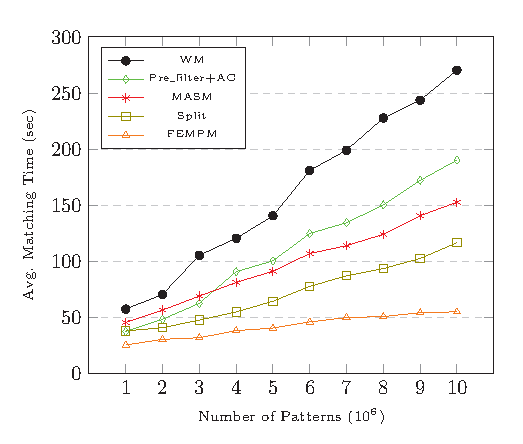
\includegraphics[height=2in, width=2.5in]{./eps/large_group}
  \caption{测试算法对于较大一组模式集的平均运行时间.}
  \label{fig:large_group}
\end{figure}

对于较大一组模式集, 测试算法的平均运行时间如图 \ref{fig:large_group} 所
示. 可以看到, 随着模式串数量由 $10^6$ 增加到 $10^7$, 每个测试算法的匹配
时间增幅分别为: $410\%$ (\textsf{WM}), $374\%$
(\textsf{Pre-filter+AC}), $238\%$ (\textsf{MASM}), $191\%$
(\textsf{Split}), $112\%$ (\textsf{FEMPM}). 每增加 $10^6$ 个模式串, 测
试算法的匹配时间的平均增加量分别为: $23.7s$ (\textsf{WM}), $17.0s$
(\textsf{Pre-filter+AC}), $12.3s$ (\textsf{MASM}),
$8.8s$(\textsf{Split}), $3.5s$ (\textsf{FEMPM}). 由此可见,
\textsf{Pre-filter+AC} 和 \textsf{WM} 算法对于较大规模的模式集表现不
佳. 这是因为, 随着模式串数量的增加, 文本串中每个位置匹配到某个模式串的
概率就会增加,这会减少过滤器的效果,导致算法性能下降。 \textsf{MASM}算
法在模式集规模大于$3 \times 10^6$时,优于 \textsf{Pre-filter+AC} 算法,
这主要归功于其所采用的模式集压缩技术和流水线化的二叉查找树良好的伸缩
性。 \textsf{Split} 算法相比其它算法 (除了 \textsf{FEMPM}) 具有更好的伸
缩性, 因为它只是从模式集中选取了一个子集(其中的每个模式串都不是其它任何
模式串的后缀)来构造DFA。

\begin{table}[!htp]
  \caption{较大一组模式集所对应AMT的节点类型统计}
  \scriptsize
  \label{tab:large_group}
  \begin{tabular}{p{25pt}p{25pt}p{25pt}p{25pt}p{20pt}p{10pt}p{30pt}p{30pt}p{20pt}p{25pt}}
 \hline
 Size &
 Map 1 &
 Map 4 &
 Map 16 &
 Map 48 &
 Map 256 &
 Single String Array &
 String Array   &
 Hash Table &
 Total\\
\hline
$1 \times 10^6$ &  38,935 &   27,428  &   6,468 &     851   &    4 &    588,343  &    240,886 &  1,027 &    903,942  \\
$2 \times 10^6$ &  85,900 &   68,973  &  17,084 &   2,141   &   20 &  1,091,527  &    496,001 &  2,015 &  1,763,661  \\
$3 \times 10^6$ & 136,054 &  117,527  &  28,092 &   3,410   &   17 &  1,547,659  &    764,359 &  2,749 &  2,599,867  \\
$4 \times 10^6$ & 189,926 &  171,155  &  40,328 &   4,716   &   23 &  1,966,326  &  1,045,558 &  3,450 &  3,421,482  \\
$5 \times 10^6$ & 247,707 &  230,163  &  83,043 &   5,989   &  38 &  2,354,308   &  1,332,896 &  3,885 &  4,228,029  \\
$6 \times 10^6$ & 304,863 &  293,591  &  65,475 &   7,169   &   49 &  2,706,094  &  1,625,261 &  4,379 &  5,006,881  \\
$7 \times 10^6$ & 366,861 &  361,695  &  77,899 &   8,434   &   53 &  3,030,673  &  1,925,027 &  4,733 &  5,775,380  \\
$8 \times 10^6$ & 429,121 &  433,708  &  90,280 &   9,660   &   62 &  3,336,765  &  2,226,879 &  5,070 &  6,531,545  \\
$9 \times 10^6$ & 494,278 &  509,992  & 102,402 &  10,833   &   72 &  3,623,407  &  2,537,413 &  5,224 &  7,283,621  \\
$1 \times 10^7$ & 558,241 &  591,455  & 115,012 &  11,922   &   79 &  3,986,683  &  2,847,277 &  5,505 &  8,026,174  \\
\hline
\end{tabular}
\end{table}

相比之下, 对于规模较大的模式集, \textsf{FEMPM} 在所有测试算法中都是最
高效的。 模式串数量每增加 $10^6$, 匹配时间仅增加2.8s多, 这主要得益
于AMT优秀的可伸缩性,使得匹配时间随着模式串数量的增加而增长地非常缓
慢。 对于较大组模式集所对应的AMT,其节点类型统计信息如
表 \ref{tab:large_group} 所示. 其中,模式串数量每增加 $10^6$,AMT中只增
加大约 $8 \times 10^5$个节点。

\section{本章小结}
\label{sec:conclusion}

本章中,我们提出了一种快速的多模式匹配引擎 \textsf{FEMPM}. 引擎由过滤模
块与核实模块组成. 过滤模块主要用于过滤掉文本串中的非匹配位置, 而核实模
块则用于核实潜在的匹配位置. 核实模块基于一种被称为自适应匹配树的数据结
构, 它可以根据模式集的特性, 自适应的调整其内部节点结构, 使其具有良好的
鲁棒性和伸缩性. 得益于此, \textsf{FEMPM} 可以很好的应用于大规模模式匹配
问题. 未来, 我们将研究更加高效的节点结构.

\begin{thebibliography}{99}

% \bibitem{Yan2016} Yan, Ruoyu. ``Combining Renyi Entropy and EWMA to
%   Detect Common Attacks in Network'' {\it International Journal of
%     Pattern Recognition and Artificial Intelligence}, 30(10),
%   pp.1650021, 2016.


% \bibitem{Xue2015} Xue, Xingsi and Wang, Yuping, ``Optimizing ontology
%   alignments through a Memetic Algorithm using both MatchFmeasure and
%   Unanimous Improvement Ratio'', {\it ARTIFICIAL INTELLIGENCE}, 223,
%   pp.65-81, 2015.

% \bibitem{Xue2016} Xue, Xingsi and Wang, Yuping, ``Using Memetic
%   Algorithm for Instance Coreference Resolution'', {\it IEEE
%     TRANSACTIONS ON KNOWLEDGE AND DATA ENGINEERING}, 223, pp.65-81,
%   2015.

% \bibitem{Kim2015} Kim, HyunJin and Choi, Kang-Il and Choi, Sang-Il,
%   ``A Memory-Efficient Deterministic Finite Automaton-Based Bit-Split
%   String Matching Scheme Using Pattern Uniqueness in Deep Packet
%   Inspection'', {\it PLOS ONE}, 10(5), 2015.


% \bibitem{Xiao2016} Guoqing Xiao, Kenli Li, Xu Zhou, Keqin
%   Li. ``Queueing Analysis of Continuous Queries for Uncertain Data
%   Streams Over Sliding Windows'' {\it International Journal of Pattern
%     Recognition and Artificial Intelligence}, 30(9), pp.1660001, 2016.

% \bibitem{Wu1994} Sun Wu and Udi Manber, ``A fast algorithm for
%   multi-pattern searching'', {\it Technical Report-94-17}, 1994.

% \bibitem{Lee2013} Tsern-Huei Lee and Nai-Lun Huang, ``A
%   pattern-matching scheme with high throughput performance and low
%   memory requirement'', {\it IEEE/ACM Transactions on Networking},
%   21(4), pp.1104--1116, 2013.

% \bibitem{Aho1975} Alfred V. Aho and Margaret J. Corasick, ``Efficient
%   string matching:An aid to bibliographic search'', {\it Commun. ACM}
%   18(6), pp.333-340, 1975.

% \bibitem{Knuth1977} Donald E. Knuth, Jr. James H. Morris, and Vaughan
%   R. Pratt, ``Fast pattern matching in strings'', {\it SIAM Journal on
%     Computing}, 6(2), pp.323–350, 1977.

% \bibitem{Boyer1977} Robert S. Boyer and J. Strother Moore, ``A fast
%   string searching algorithm'', {\it Commun. ACM}, 20(10), pp.762–772,
%   1977.

% \bibitem{Zhang2016} Lungan Zhang, Liangxiao Jiang, Chaoqun Li. ``A New
%   Feature Selection Approach to Naive Bayes Text Classifiers'' {\it
%     International Journal of Pattern Recognition and Artificial
%     Intelligence}, 30(9), pp.1650003 2016.

% \bibitem{Tang2015} Guoyu Tang, Yunqing Xia, Erik Cambria, Peng Jin,
%   Thomas Fang Zheng. ``Document Representation with Statistical Word
%   Senses in Cross-Lingual Document Clustering'' {\it International
%     Journal of Pattern Recognition and Artificial Intelligence},
%   30(9), pp.1559003, 2015.

% \bibitem{Tuck2004} N. Tuck, T. Sherwood, B. Calder, and G. Varghese,
%   ``Deterministic memory-efficient stringmatching algorithms for
%   intrusion detection'', {\it Twenty-third AnnualJoint Conference of
%     the IEEE Computer and Communications Societies}, Vol 4,
%   pp.2628–2639, 2004.

% \bibitem{Bremler2011} A. Bremler-Barr, Y. Harchol, and D. Hay,
%   ``Space-time tradeoffs in software-based deep packet inspection'',
%   {\it In High Performance Switching and Routing (HPSR), IEEE 12th
%     International Conference on}, pp.1–8, 2011.

% \bibitem{Ramakrishnan2010} Ramakrishnan Kandhan, Nikhil Teletia, and
%   Jignesh M. Patel, ``Sigmatch: Fast and scalable multi-pattern
%   matching'', {\it Proceedings of the VLDB Endowment}, 3(1),
%   pp.1173–1184, 2010.

% \bibitem{Zhou2007} Zongwei Zhou, Yibo Xue, Junda Liu, Wei Zhang, and
%   Jun Li, ``MDH: A high speed multi-phase dynamic hash string matching
%   algorithm for large-scale pattern set'', {\it Information and
%     Communications Security Springer}, pp.201-215, 2007.

% \bibitem{Zhan2014} P. Zhan, W. Yuping, and X. Jinfeng, ``An improved
%   multi-pattern matching algorithm for large-scale pattern sets'',
%   {\it In Computational Intelligence and Security (CIS), Tenth
%     International Conference on}, pp.197–200, 2014.

% \bibitem{Zhang2009} Baojun Zhang, Xiaoping Chen, Xuezeng Pan, and
%   Zhaohui Wu, ``High concurrence wu-manber multiple patterns matching
%   algorithm'', {\it Proceedings of the International Symposium on
%     Information Process}, pp.404-409, 2009.

% \bibitem{Choi2011} Yoon-Ho Choi, Moon-Young Jung, and Seung-Woo Seo,
%   ``A fast pattern matching algorithm with multi-byte search unit for
%   highspeed network security'', {\it Computer Communications}, 34(14),
%   pp.1750–1763, 2011.

% \bibitem{Le2013} Hoang Le and V.K. Prasanna, ``A memory-efficient and
%   modular approach for large-scale string pattern matching'', {\it
%     Computers, IEEE Transactions on}, 62 (5), pp.844–857, 2013.

% \bibitem{Moraru2013} Iulian Moraru and David G. Andersen, ``Exact
%   pattern matching with feed-forward bloom filters'', {\it Journal of
%     Experimental Algorithmics}, Vol.17, pp.3-4, 2013.

% \bibitem{Karp1987} R. M. Karp and M. O. Rabin, ``Efficient randomized
%   patternmatching algorithms'', {\it IBM Journal of Research and
%     Development}, 31 (2), pp.249-260, 1987.

% \bibitem{Agarwal2013} K. Agarwal and R. Polig, ``A high-speed and
%   large-scale dictionary matching engine for information extraction
%   systems'',{\it Application-Specific Systems, Architectures and
%     Processors (ASAP), IEEE 24th International Conference on},
%   pp.59–66, 2013.

% \bibitem{Zhang2015} Hongli Zhang, Dongliang Xu, Zhihong Tian, and
%   Yujian Fan, ``An efficient parallel algorithm for exact
%   multi-pattern matching'', {\it Security And Communication Networks},
%   8 (9), pp.1688–1697, 2015.

% \bibitem{I2015} Tomohiro I, Takaaki Nishimoto, Shunsuke Inenaga, Hideo
%   Bannai, and Masayuki Takeda, ``Compressed automata for dictionary
%   matching'', {\it Theoretical Computer Science}, Vol.578, pp.30–41,
%   2015.

% \bibitem{Khancome2013} Chouvalit Khancome and Veera Boonjing, ``A new
%   linear-time dynamic dictionary matching algorithm'', {\it Computing
%     And Informatics}, 32 (5), pp.897–923, 2013.

% \bibitem{Amir2015} Amihood Amir, Avivit Levy, Ely Porat, and B. Riva
%   Shalom, ``Dictionary matching with a few gaps'', {\it Theoretical
%     Computer Science}, Vol.589, pp.34–46, 2015.

% \bibitem{Neuburger2012} Shoshana Neuburger and Dina Sokol. ``Succinct
%   2d dictionary matching'', {\it Algorithmica}, 65 (3), pp.662–684,
%   2012.

% \bibitem{Leis2013} V. Leis, A. Kemper, and T. Neumann. ``The adaptive
%   radix tree: Artful indexing for main-memory databases'', {\it In
%     Data Engineering(ICDE), IEEE 29th International Conference on},
%   pp.38–49, 2013.

% \bibitem{Ramakrishna1997} M. V. Ramakrishna and Justin
%   Zobel. ``Performance in practice of string hashing functions'', {\it
%     In Proceedings of the Fifth International Conference on Database
%     Systems for Advanced Applications (DASFAA)}, pp.215–224, 1997.

% \bibitem{Kim2015} Kim, HyunJin AND Choi, Ki AND Choi,
%   Si. ``A Memory-Efficient Deterministic Finite Automaton-Based
%   Bit-Split String Matching Scheme Using Pattern Uniqueness in Deep
%   Packet Inspection'', {\it PLOS ONE}. vol.10, pp.1-24, 2015.

% \bibitem{pizzachil} {\it http://pizzachil.dcc.uchile.cl/}

\end{thebibliography}  


\vspace*{-0.01in}
%\vspace*{-0.3in}
\noindent
\rule{12.6cm}{.1mm}

\end{document}

%%% Local Variables:
%%% mode: latex
%%% TeX-master: t
%%% End:

%%% Local Variables:
%%% mode: latex
%%% TeX-master: t
%%% End:
